
In this document, we discuss a draft of an IVOA standard data model for
describing the provenance of astronomical data. 
We follow the definition of provenance as proposed by the W3C \citep{std:W3CProvDM}, i.e. that provenance is ``information about entities, activities, and people involved in producing a piece of data or thing, which can be used to form assessments about its quality, reliability or trustworthiness''.

In astronomy, such entities are generally datasets composed of VOTables, FITS
files, database tables or files containing values (spectra, light curves), logs,
parameters.
The activities correspond to processes like an observation, a
simulation, processing steps (image stacking, object extraction, etc.), execution of data analysis code, publication, etc.
The people involved can be for example individual persons (observer, publisher, etc.), groups or organisations. An example for activities, entities and agents as they can be discovered backwards in time is given in Figure~\ref{fig:example-workflow}.

The links between the Provenance DM and other IVOA data models will be discussed in Section~\ref{sec:dmlinks}. We note here that the provenance of simulated data is included in the Simulation DM \citep[SimDM,][]{std:SimDM}. Therefore we also give a mapping between SimDM and the Provenance DM in Section~\ref{sec:dmlinks}.

We also introduce a few constructs from the ProvONE data model \citep{ProvONE}, that proposes extensions to W3C PROV for scientific workflow provenance. We discuss the mapping between ProvONE and the Provenance DM in Appendix~\ref{sec:dmlinks}.

\begin{figure}[ht]
\centering
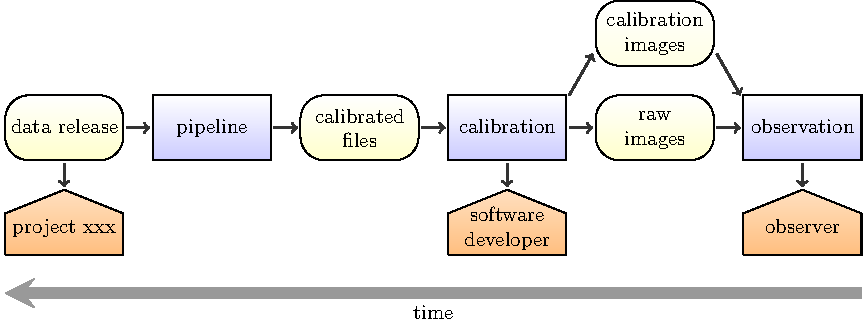
\includegraphics[width=1\textwidth]{workflow-backwards.pdf}
\caption[Example graph of provenance discovery]{An example graph of provenance discovery. Starting with a released dataset (left), the involved activities (blue boxes), 
progenitor entities (yellow rounded boxes) and responsible agents (orange pentagons) are 
discovered.}
\label{fig:example-workflow}
\end{figure}


%including extraction of data from 
%databases or even the flow of scientific proposals from application to 
%acceptance, including scheduling of the observations proposed therein.
%Provenance information could also be used to check internal processes,
%e.g., whether a proposal was approved by a person from a certain committee,
%or whether the time span between application and acceptance or rejection
%does not extend a certain period, etc... 


\subsection{Goal of the provenance model}
\label{sec:goals}

The goal of this Provenance DM is to describe how provenance information
can be modelled, stored and exchanged. Its scope
is mainly modelling of the flow of data, of the relations between data,
and of processing steps. The currently discussed Provenance DM is sufficiently abstract that its core pattern (see Section~\ref{sec:core_model}) could be applied to any kind of process using either observation or simulation data.
It could also be used to describe the workflow for observation proposals or the publication of scientific articles based on (astronomical) data.

Characteristics of observation activities such as ambient conditions and
instrument characteristics provide useful information to asses the quality and reliability of the generated entities. 
Experimental configuration or contextual information during
the execution of processing activities (computer structure, nodes, operating
system used, etc) can also be relevant for the description of the main entities generated. This complementary information should be included in the form of metadata or additional entities and connected to an activity (see Section~\ref{sec:extended_model}). However, the precise structure and modelling of those characteristics is out of the scope of this document. 

In general, the model shall capture information in a machine-readable way that would enable a scientist who has no prior knowledge about a dataset to get more background information. 
This will help the scientist to decide if the dataset 
is adequate for her research goal, assess its quality and get enough information
to be able to trace back its history as far as required or possible. 

Provenance information may be recorded in minute detail or by using coarser
elements, depending on the intended usage and the desired level of detail
for a specific project that records provenance. 
This granularity depends on the needs of the project and the intended usage when implementing a system to track provenance information.
% NOTE: maybe we need to define minimal requirements of what needs to be included as provenance information?

The following list is a collection of tasks which the Provenance DM should help to solve. They are flagged with [S] for problems which are more interesting for the end user of datasets (usually a scientist) and with [P] for tasks that are probably more important for data producers and publishers.
More specific use cases in the astronomy domain for different types of datasets and workflows along with example implementations are given in the Implementation Note \citep{std:ProvenanceImplementationNote}.


\paragraphlb{A: Tracking the production history [S]}
        Find out which steps were taken to produce a dataset and list the
        methods\slash{}tools\slash{}software that were involved. Track the
        history back to the raw data files \slash{} raw images, show the
        workflow (backwards search), or return a list of progenitor datasets.

        \noindent Examples: 
        \begin{itemize}
            \item Is an image already calibrated?
What about dark field subtraction? Were foreground stars removed? Which technique
was used?  
            \item Is the background noise of atmospheric muons still present in my neutrino data sample?  
        \end{itemize}

        We do not go as far as to consider easy reproducibility as a use case -- this would be too ambitious. But at least the 
        major steps undertaken to create a piece of data should be recoverable.


\paragraphlb{B: Attribution and contact information [S]}
        Find the people involved in the production of a dataset,
        the people\slash{}organizations\slash{}institutes that need to be cited
        or can be asked for more information.

        \noindent Examples: 
        \begin{itemize}
            \item I want to use an image for my own work -- who was involved in
creating it? Who do I need to cite or who can I contact to get this information? Is a license attached to the data? 
            \item I have a question about column xxx in a data
table. Who can I ask about that?  
            \item Who should be cited or acknowledged if I use this data in my work?
        \end{itemize}


\paragraphlb{C: Locate error sources [S, P]}
        Find the location of possible error sources in the generation of a dataset.

        \noindent Examples:
        \begin{itemize}
            \item I found something strange in an image. Where does
the image come from? Which instrument was used, with which characteristics,
etc.? Was there anything strange noted when the image was taken?  
            \item Which pipeline version was used -- the old one
with a known bug for treating bright objects or a newer version?  
            \item This light curve doesn't look quite right. How was
the photometry determined for each data point?  
        \end{itemize}


\paragraphlb{D: Quality assessment [P]}
        Judge the quality of an observation, production step or dataset.
        
        \noindent Examples:
        \begin{itemize}
            \item Since wrong calibration images may increase the
number of artifacts on an image rather than removing them, knowledge about
the calibration image set will help to assess the quality of the calibrated
image.  
        \end{itemize}
      

\paragraphlb{E: Search in structured provenance metadata [P, S]}
        This would allow one to also do a ``forward search'', i.e. locate derived datasets or outputs, e.g. finding all images produced by a certain processing step or derived from data which were taken by a given facility.
        
        \noindent Examples:
        \begin{itemize}
            \item Give me more images that were produced using the same pipeline.  
            \item Give me an overview on all images reduced with the same calibration dataset.  
            \item Are there any more images attributed to this observer?  
            \item Which images of the Crab Nebula are of good quality and were produced within the last 10 years by someone not from ESO or NASA?
            \item Find all datasets generated using this given algorithm for this given step of the data processing.
          % add another specific use case for tracking scientific productivity?
        \end{itemize}

        This task is probably the most challenging. It also includes tracking the history of data items as in A, but we still have listed this task separately, since we may decide that we can't keep this one, but we definitely want A.
